\documentclass[Ex4_Zusammenfassung.tex]{subfiles}


\begin{document}
\clearpage
\section{Übersicht des Elementarteilchen--Zoos}
\textbf{von \hein \& \soeren}\\

\begin{table}[H]
	\centering
	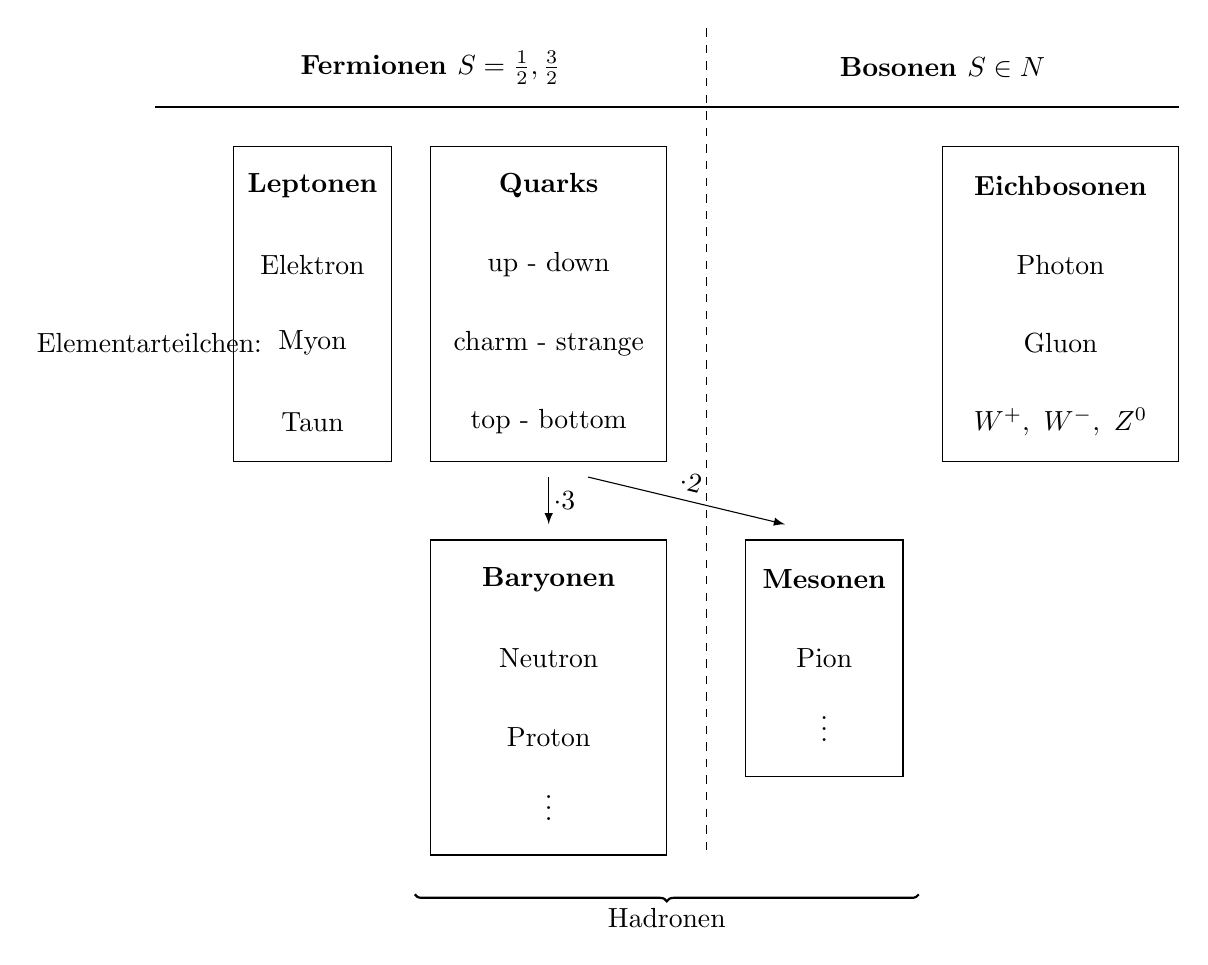
\begin{tikzpicture}
		% Lines
		\draw [thick] (-1,0) -- (12,0);
		\draw [dashed] (6, 1) -- (6, -9.5);
		%Header
		\node at (2.5, 0.5) (F) {\textbf{Fermionen $\lp S= \frac{1}{2} , \frac{3}{2} \rp$ }};
		\node at (9, 0.5) (Bo) {\textbf{Bosonen $\lp S \in \mathbb{N} \rp $}};
		%sidenote
		\node at (-1.5, -3) (ET) [text width=2cm]{Elementarteilchen:};
		% Leptonen
		\node at (1, -1) (L) {\textbf{Leptonen}};
		\node at (1,-2) (el) {Elektron};
		\node at (1, -3) (mu) {Myon};
		\node at (1, -4) (ta) {Taun};
		\draw (0, -4.5) rectangle (2, -0.5);
		%Quarks
		\node at (4, -1) (Q) {\textbf{Quarks}};
		\node at (4, -2) (ud) {up - down};
		\node at (4, -3) (cs) {charm - strange};
		\node at (4, -4) (tb) {top - bottom};
		\draw (2.5, -4.5) rectangle (5.5, -0.5);
		%Baryonen
		\draw [->, >=latex] (4, -4.7) -- (4, -5.3) node [midway, xshift=0.2cm] (times3) {$\cdot 3$};
		\node at (4, -6) (B) {\textbf{Baryonen}};
		\node at (4, -7) (N) {Neutron};
		\node at (4, -8) (P) {Proton};
		\node at (4, -8.8) (ddd) {$\vdots$};
		\draw (2.5, -9.5) rectangle (5.5, -5.5);
		%Mesonen
		\draw [->, >=latex] (4.5, -4.7) -- (7, -5.3) node [midway, above, sloped] (times2) {$\cdot 2$};
		\node at (7.5, -6) (M) {\textbf{Mesonen}};
		\node at (7.5, -7) (Pi) {Pion};
		\node at (7.5, -7.8) (ddd2) {$\vdots$};
		\draw (6.5, -8.5) rectangle (8.5, -5.5);
		%Eichbosonen
		\node at (10.5, -1) (E) {\textbf{Eichbosonen}};
		\node at (10.5, -2) (Ph) {Photon};
		\node at (10.5, -3) (Gl) {Gluon};
		\node at (10.5, -4) (WZ) {$W^+,\ W^-,\ Z^0$};
		\draw (9, -4.5) rectangle (12, -0.5);
		%underbrace
		\draw [thick, decoration={brace, mirror, raise=0.5cm}, decorate] (2.3, -9.5) -- (8.7, -9.5) node [pos=0.5,anchor=north,yshift=-0.55cm] {Hadronen}; 
	\end{tikzpicture}
	\caption{Übersicht des Elementarteilchen-Zoos}
\end{table}

\subsection{Anmerkungen}
\begin{itemize}
	\item Es gibt 8 unabhängige Gluonen, die sich in ihrer Farbladung unterscheiden
	\item Das Higgs--Boson ist ein weiteres Elementarteilchen, das sich keiner der 3 Gruppen zuordnen lässt und Teil des Higgs--Feldes ist. (Annahme: durch Wechselwirkung mit dem Higgsfeld erhalten Teilchen ihre Masse.)
\end{itemize}

\section{Leptonen}
\begin{itemize}
	\item Es gibt 3 Generationen: $e,\ \mu,\ \tau$
	\item In jeder Generation ein Teilchen mit $q=-e$ und eines mit $q=0$ sowie deren Antiteilchen
	\item Antiteilchen haben entgegengesetztes Vorzeichen bei Ladung und Leptonenzahl
\end{itemize}

\begin{table}[H]
	\centering
	$
	\begin{array}{cccc}
		\text{Generation} & q=-1 & q=0 & \text{Leptonenzahl } \lp = n_L - n_{\bar{L}} \rp \\ \hline
		1 & e^- & \nu_e & L_e = 1,\ L_\mu = 0,\ L_\tau = 0 \\ 
		2 & \mu^- & \nu_\mu & L_e = 0,\ L_\mu = 1,\ L_\tau = 0 \\ 
		3 & \tau^- & \nu_\tau & L_e = 0,\ L_\mu = 0,\ L_\tau = 1
	\end{array} 
	$ 
	\captionof{table}{Übersicht der 3 Leptonen--Generationen und ihrer Eigenschaften}
\end{table}

Die Antileptonen werden wie folgt notiert: $e^+,\ \mu^+,\ \tau^+,\ \overline{\nu}_e,\ \overline{\nu}_\mu,\ \overline{\nu}_\tau$. Sie haben \textbf{negative} Leptonenzahl.

\bsp{
	Myon zerfällt zu einem Elektron und zwei Neutrinos:
	
	\begin{table}[H]
		\centering
		$
		\begin{array}{c|rcrrr}
		& \mu^- & \rightarrow & e^-\ & +\ \overline{\nu}_e\ & +\ \nu_\mu \\ \hline
		q & -1 &  & -1 & 0 & 0 \\ 
		L_e & 0 &  & 1 & -1 & 0 \\ 
		L_\mu & 1 &  & 0 & 0 & 1
		\end{array} 
		$
		\captionof{table}{Myonenzerfall}
	\end{table}
	
	Ladung und Leptonenzahl bleiben \textbf{erhalten}. Die Masse der Produkte darf die des Edukts nicht überschreiten (''kinematisch erlaubt'').
}
\section{Quarks}
Für Quarks und Hadronen (Quark--Komposita) führen wir weitere Quantenzahlen ein. Da up-- und down--Quark sehr ähnliche Eigenschaften (Masse) besitzen, können sie durch eine gemeinsame Quantenzahl beschrieben werden (wird in folgenden Kapiteln präzisiert).
\begin{table}[H]
	\centering
	$
	\begin{array}{clrrrrrr}
		\text{Generation} & \text{Flavour} & \text{q} & I_3 & S & C & B & T\\ \hline
		\multirow{2}{*}{1} 	& d\ (down) & - \nicefrac{1}{3} & - \nicefrac{1}{2} &&&&\\
										   & u\ (up) & \nicefrac{2}{3} & \nicefrac{1}{2} &&&& \\
		\multirow{2}{*}{2} 	& s\ (strange) & - \nicefrac{1}{3} && -1 &&\text{\huge0}&\\
										   & c\ (charm) & \nicefrac{2}{3} &&& 1 && \\
		\multirow{2}{*}{3} 	& b\ (bottom) & - \nicefrac{1}{3} &&\text{\huge0}&& -1 &\\
										   & t\ (top) & \nicefrac{2}{3} &&&&& 1								   							   
	\end{array}
	$
	\caption{Übersicht der 3 Quark-Generationen und deren Eigenschaften}
\end{table}

Hierbei steht $I_3$ (auch $I_z$) für die z--Projektion des sog. Isospins $I$ und S, C, B, T für weitere Quantenzahlen: Strangeness, Charmness, Bottomness und Topness. \\

Antiquarks haben umgekehrtes Vorzeichen bei Ladung und Quantenzahlen/Isospin. $I_3$, S, C, B, T sind Flavour--Quantenzahlen:
\subsection{Flavour--Quantenzahlen $I_3,\ S,\ C,\ B,\ T$}
Die z--Projektion des Isospins ist definiert durch
\begin{align}
		&I_3 = \frac{1}{2} \lp \lp n_u - n_{\overline{u}} \rp - \lp n_d - n_{\overline{d}} \rp \rp 
		\intertext{Hieraus folgt für up-- und down--Quarks:}
		&up-Quark:\ I_3 = \frac{1}{2};\ down-Quark:\ I_3=-\frac{1}{2}
\end{align}
\begin{align}
	C &= n_c - n_{\overline{c}} \rightarrow charm-Quark:\ C=1\\
	S &= n_s - n_{\overline{s}} \rightarrow strange-Quark:\ S=-1\\
	T &= n_t - n_{\overline{t}} \rightarrow top-Quark:\ T=1\\
	B &= n_b - n_{\overline{b}} \rightarrow bottom-Quark:\ B=-1
\end{align}
wobei $n$ jeweils die Anzahl der (Anti--)Quarks beschreibt.

\subsection{Farbladung}
Die Farbladung ist eine weitere Quantenzahl. 
Quarks können 3 verschiedene Farbladungen annehmen: $r,\ g,\ b$ (rot, grün, blau)\\
Antiquarks können 3 Antifarben annehmen: $\overline{r},\ \overline{g},\ \overline{b}$ (cyan, magenta, gelb)\\

Alle gebundenen Zustände sind farbneutral (\textbf{Confinement-Hypothese}).\\
Dies kann auf 2 Arten erreicht werden:
\begin{itemize}
	\item Kombination von Quark und Antiquark (Mesonen)\\
	$\rightarrow$ Farbe + Antifarbe = Neutral\\
	\quad -- Zerfallen in Sekundenbruchteilen
	\item Kombination aller 3 Farben, also 3 Quarks (Baryonen)\\
	$\rightarrow$ $r+g+b=weiß$ (neutral)
\end{itemize}

Gluonen tragen jeweils eine Farb- und Antifarbladung.\\
$\rightarrow\ 3^2 = 9$ Kombinationsmöglichkeiten\\
$\rightarrow$ davon ist aber eine neutral $\rightarrow$ 8 Möglichkeiten

\begin{itemize}
	\item Leptonen unterliegen der schwachen WW, der Gravitation und -- falls sie geladen sind -- der elektromagnetischen Wechselwirkung.
	\item Quarks unterliegen allen Wechselwirkungen
\end{itemize}
\end{document}